% =============================================================================
% exhibits.tex
%
% Every figure and table of the paper, with draft captions and notes, in the
% order planned in horario_verao/PAPER.md. The bodies are generated:
%   figures  analysis/code/20_figures.R  -> analysis/output/graphs/*.pdf
%   tables   analysis/code/21_tables.R   -> analysis/output/tables/*.tex
% Captions and notes live here (and later in the manuscript), never in the
% generated files. Figures are saved at the size they print at: \textwidth of
% a 12pt article with 1in margins (6.5in), so nothing is rescaled.
%
% Compile from this folder: latexmk -pdf exhibits.tex
% =============================================================================
\documentclass[12pt]{article}
\usepackage[margin=1in]{geometry}
\usepackage[T1]{fontenc}
\usepackage{lmodern}
\usepackage{amsmath}
\usepackage{booktabs}
\usepackage{graphicx}
\usepackage[labelfont=bf, font=small, justification=raggedright,
            singlelinecheck=false]{caption}
\usepackage{threeparttable}
\usepackage{float}

\graphicspath{{../analysis/output/graphs/}}
\newcommand{\tabdir}{../analysis/output/tables}
% Table notes: small, flush left, full width of the table.
\newcommand{\tabnote}[1]{\begin{tablenotes}[flushleft]\footnotesize\item \textit{Notes:} #1\end{tablenotes}}
\newcommand{\fignote}[1]{\par\vspace{4pt}{\footnotesize\noindent\textit{Notes:} #1\par}}
\renewcommand{\topfraction}{0.9}
\renewcommand{\textfraction}{0.07}
\renewcommand{\floatpagefraction}{0.8}

\begin{document}

\section*{Specification}

Every estimate in log points comes from a Poisson regression on the panel of
23 states by day,
\begin{equation}
  y_{sd} = \exp\big(\beta\, T_s \times W_d \times A_d + \alpha_{s,w(d)} + \gamma_{s,t(d)} + \delta_d\big)\,\varepsilon_{sd},
  \label{eq:main}
\end{equation}
where $y_{sd}$ counts events in state $s$ on day $d$ in one clock hour defined
relative to standard-time sunset or sunrise at the municipal seat; $T_s$ marks
the 11 states with DST in every season from 2008/09 to 2018/19; $W_d$ marks the
summer window (15 November to 14 February); $A_d$ marks seasons after abolition
(2019/20 to 2023/24); and the fixed effects are state by window, state by season
and date. Standard errors are clustered by state.

\clearpage
% ── Main text ────────────────────────────────────────────────────────────────

\begin{figure}[p]
  \centering
  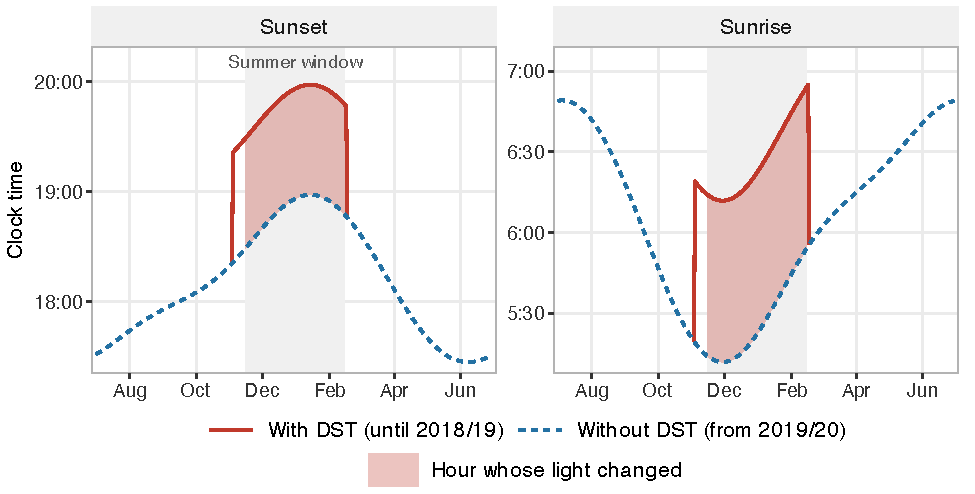
\includegraphics{fig_design.pdf}
  \caption{Clock time of sunset and sunrise with and without daylight saving time}
  \label{fig:design}
  \fignote{S\~ao Paulo, July 2018 to June 2019. The solid line is the clock
  time under the DST in force that season (4 November to 16 February); the
  dashed line is the clock time without DST, the rule since 2019/20. The grey
  band is the summer window used in every season. The shaded hour after
  standard-time sunset was light with DST and is dark without it; the hour
  after standard-time sunrise is the reverse.}
\end{figure}

\begin{figure}[p]
  \centering
  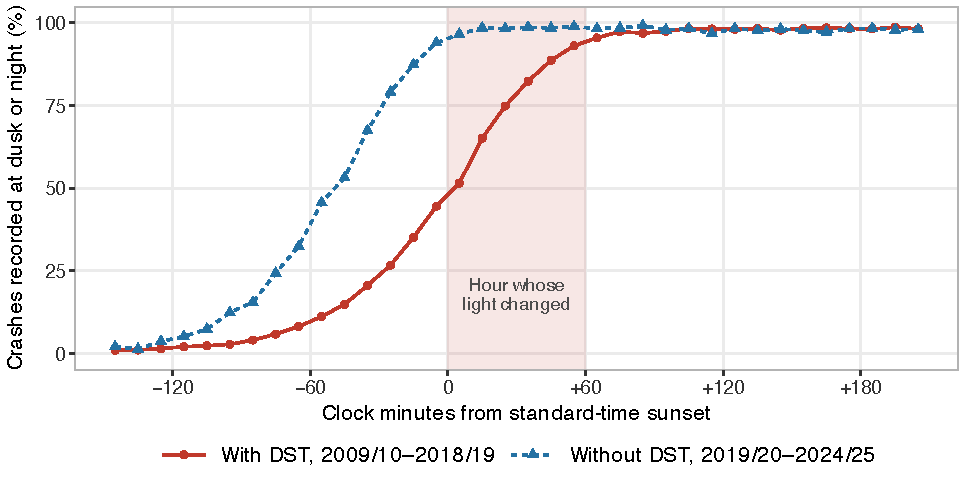
\includegraphics{fig_first_stage.pdf}
  \caption{Crashes the highway police recorded at dusk or night}
  \label{fig:first-stage}
  \fignote{Federal highway crashes in the 11 treated states, summer window.
  Share the police officer recorded as dusk or night, by 10-minute bin of
  clock time minus standard-time sunset at the municipality of the crash. The
  shaded hour is the hour whose light changed with abolition.}
\end{figure}

\begin{figure}[p]
  \centering
  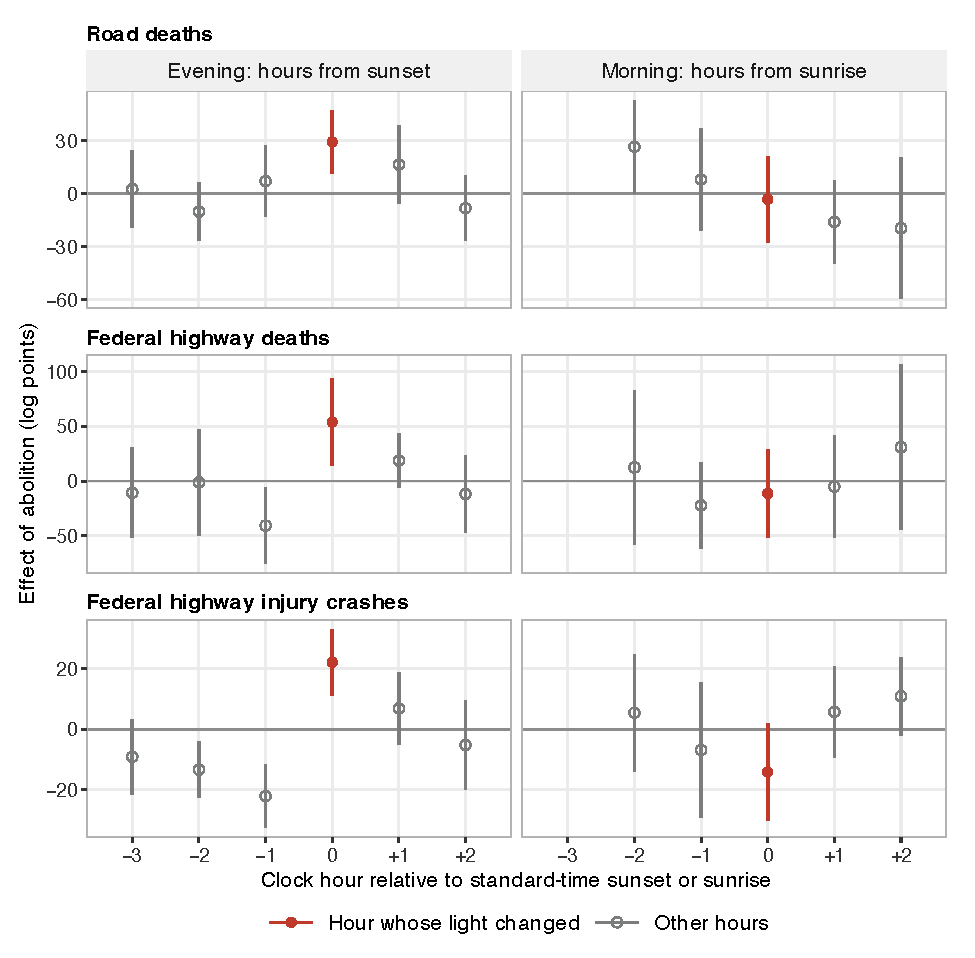
\includegraphics{fig_hours_from_sunset.pdf}
  \caption{Effect of abolition by hour relative to sunset and sunrise}
  \label{fig:hours}
  \fignote{Each point is $\beta$ from equation~(\ref{eq:main}) estimated
  separately for one clock hour, with its 95 percent confidence interval. Hour
  0 is the 60 minutes after standard-time sunset (left) or sunrise (right),
  the hour that turned dark or light; hour $-1$ is the 60 minutes before.}
\end{figure}

\begin{figure}[p]
  \centering
  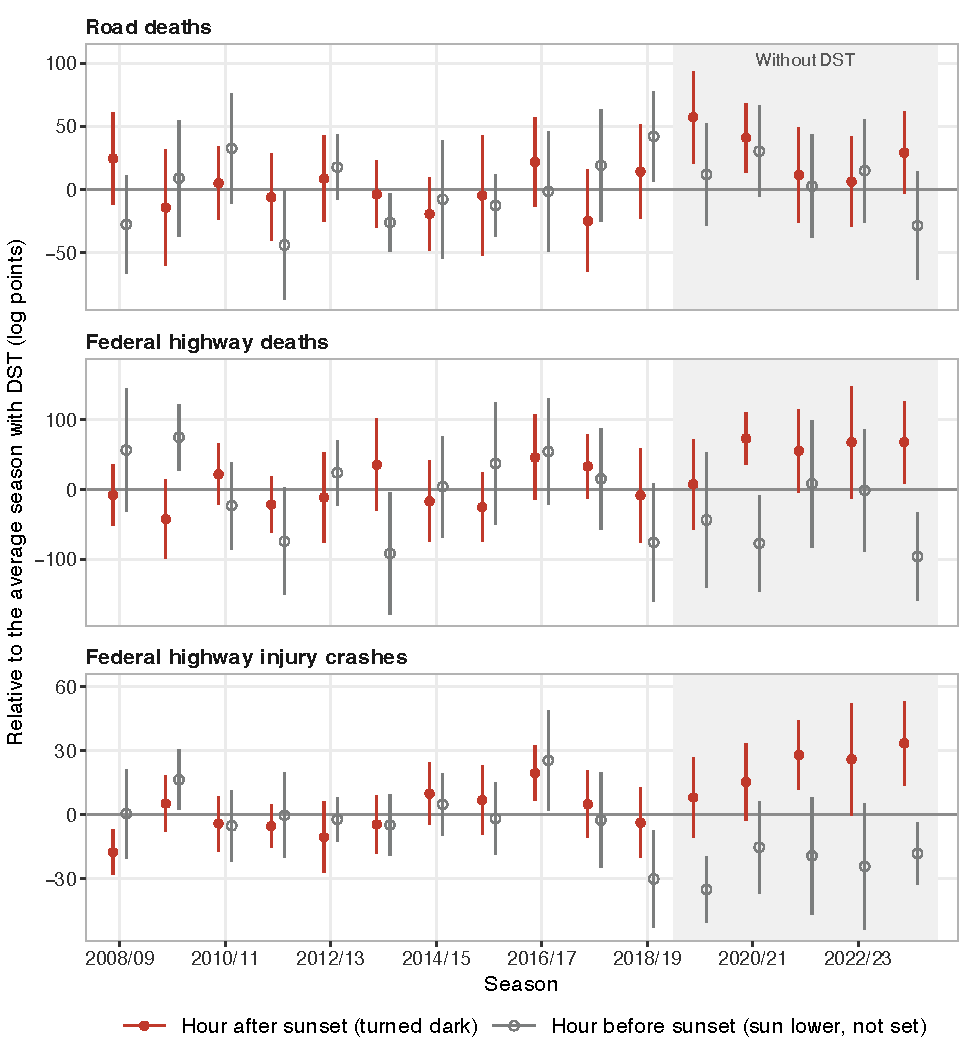
\includegraphics{fig_event_study.pdf}
  \caption{The hour after sunset and the hour before, season by season}
  \label{fig:event-study}
  \fignote{Equation~(\ref{eq:main}) with $T_s \times W_d$ interacted with each
  season instead of with $A_d$; 2018/19, the last season with DST, is the
  reference. 95 percent confidence intervals. The shaded seasons had no DST.}
\end{figure}

\begin{table}[p]
  \centering
  \caption{Events per summer by group, window and period}
  \label{tab:descriptives}
  \begin{threeparttable}
    \small\setlength{\tabcolsep}{3.5pt}
    \input{\tabdir/tab_descriptives.tex}
    \tabnote{Average count per season. Before: 2008/09 to 2018/19 (11
    seasons); after: 2019/20 to 2023/24 (5 seasons). Summer window: 15
    November to 14 February; off-season: 1 April to 31 August. Road deaths
    are deaths on a public road from death certificates; federal highway
    counts are from the federal highway police. Only events with a recorded
    clock time.}
  \end{threeparttable}
\end{table}

\begin{table}[p]
  \centering
  \caption{The hour that turned dark and the hour that turned light}
  \label{tab:main}
  \begin{threeparttable}
    \small
    \input{\tabdir/tab_main.tex}
    \tabnote{Estimates of $\beta$ in equation~(\ref{eq:main}), standard
    errors clustered by state in parentheses. The permutation p-value is the
    share of 999 random sets of 11 treated states whose estimate is at least as
    large in absolute value. Linear model: the same specification estimated by
    least squares on counts, effect as a percent of the treated states' summer
    mean before abolition; its p-value is from a wild cluster bootstrap (Webb
    weights, 9,999 draws, null imposed).}
  \end{threeparttable}
\end{table}

\begin{table}[p]
  \centering
  \caption{Pedestrians and other road users in the hour after sunset}
  \label{tab:pedestrians}
  \begin{threeparttable}
    \small
    \input{\tabdir/tab_pedestrians.tex}
    \tabnote{Equation~(\ref{eq:main}) for the hour after standard-time sunset,
    estimated separately for events with a pedestrian victim and for all
    others. Panel C comes from one stacked model. Inference as in
    Table~\ref{tab:main}. Excess events are observed minus predicted
    without abolition, in the treated states' summer windows after 2019.}
  \end{threeparttable}
\end{table}

\begin{table}[p]
  \centering
  \caption{Excess events per summer after abolition}
  \label{tab:excess}
  \begin{threeparttable}
    \small
    \input{\tabdir/tab_excess.tex}
    \tabnote{Events per summer in the treated states after abolition minus
    those predicted without it, from one model stacking the seven hours with
    every fixed effect of equation~(\ref{eq:main}) interacted with the hour.
    Delta-method standard errors in parentheses. The whole day comes from a
    separate model. Only events with a recorded clock time, so the counts
    are lower bounds.}
  \end{threeparttable}
\end{table}

\begin{table}[p]
  \centering
  \caption{Traffic volume and risk per vehicle on federal highways}
  \label{tab:volume}
  \begin{threeparttable}
    \small
    \input{\tabdir/tab_traffic_volume.tex}
    \tabnote{Log points, standard errors clustered by state in parentheses.
    Column 1: equation~(\ref{eq:main}) on hourly vehicle counts at continuous
    counting stations, with station fixed effects; no station is counted both
    before and after abolition. Columns 2 and 4: as in Table~\ref{tab:main}.
    Per vehicle: crash or death estimate minus the volume estimate.}
  \end{threeparttable}
\end{table}

\begin{table}[p]
  \centering
  \caption{The hour after sunset under other choices, and hours whose light did not change}
  \label{tab:robustness}
  \begin{threeparttable}
    \small\setlength{\tabcolsep}{5pt}
    \input{\tabdir/tab_robustness.tex}
    \tabnote{Panel A: equation~(\ref{eq:main}) with one change per row;
    standard errors clustered by state. The state-by-day row compares the hour
    with hours 3 to 5 before and 2 to 4 after sunset of the same state and
    day. The joint test is a Wald test that the
    ten season coefficients before 2018/19 in Figure~\ref{fig:event-study} are
    zero. Panel B: counterfactual fitted on untreated state-days only, with
    week and day-of-week effects; 95 percent intervals from 299 draws of a
    state bootstrap. Panel C: midday is at least three hours after sunrise
    and more than three hours before sunset; night is at least three hours
    after sunset or more than two hours before sunrise.}
  \end{threeparttable}
\end{table}

\clearpage
% ── Appendix ─────────────────────────────────────────────────────────────────

\begin{figure}[p]
  \centering
  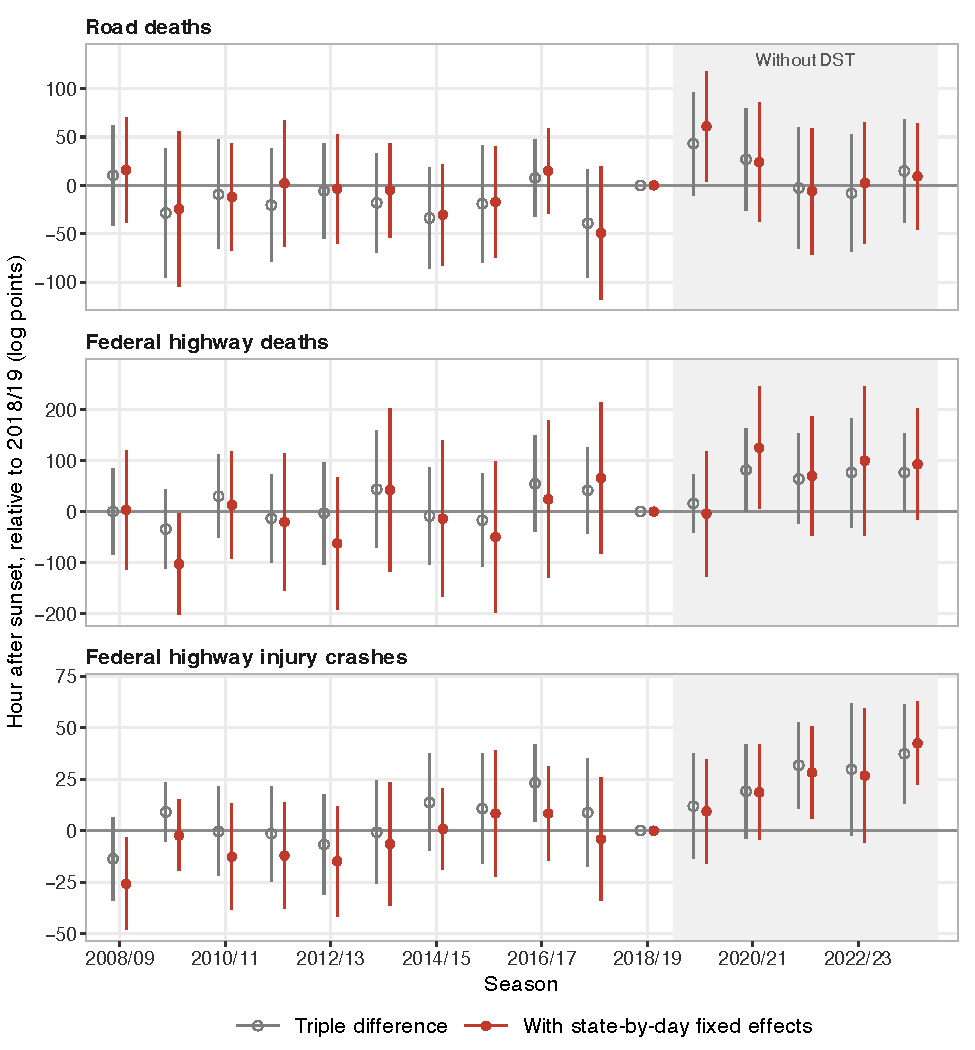
\includegraphics{fig_within_day.pdf}
  \caption{The hour after sunset with state-by-day fixed effects}
  \label{fig:within-day}
  \fignote{Grey: the hour after sunset in Figure~\ref{fig:event-study}. Red:
  the same hour estimated against hours 3 to 5 before and 2 to 4 after sunset
  of the same state and day. 95 percent confidence intervals; reference season
  2018/19.}
\end{figure}

\begin{figure}[p]
  \centering
  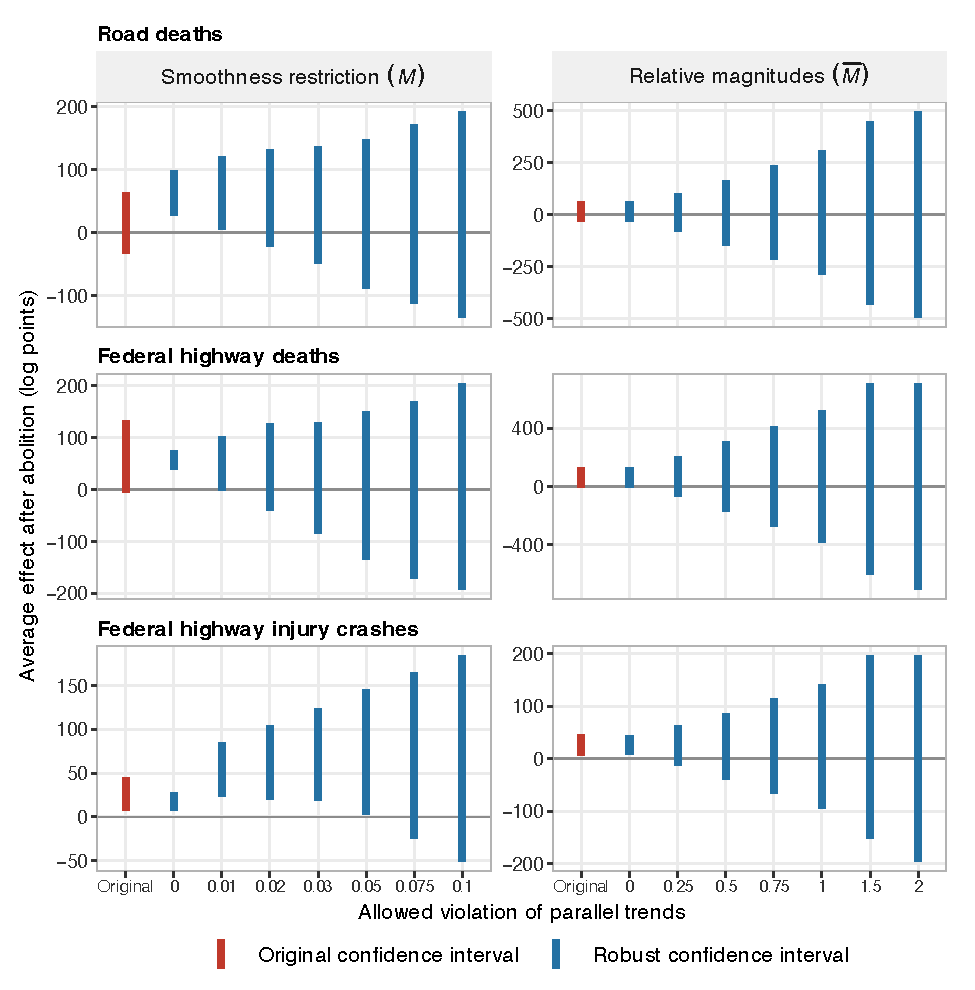
\includegraphics{fig_honestdid.pdf}
  \caption{Sensitivity to violations of parallel trends}
  \label{fig:honestdid}
  \fignote{95 percent confidence intervals for the average effect over the
  five seasons after abolition in the hour after sunset (Rambachan and Roth,
  2023). Left: the slope of the violation may change by at most $M$ between
  seasons. Right: the violation after abolition is at most $\bar M$ times the
  largest one before it.}
\end{figure}

\begin{figure}[p]
  \centering
  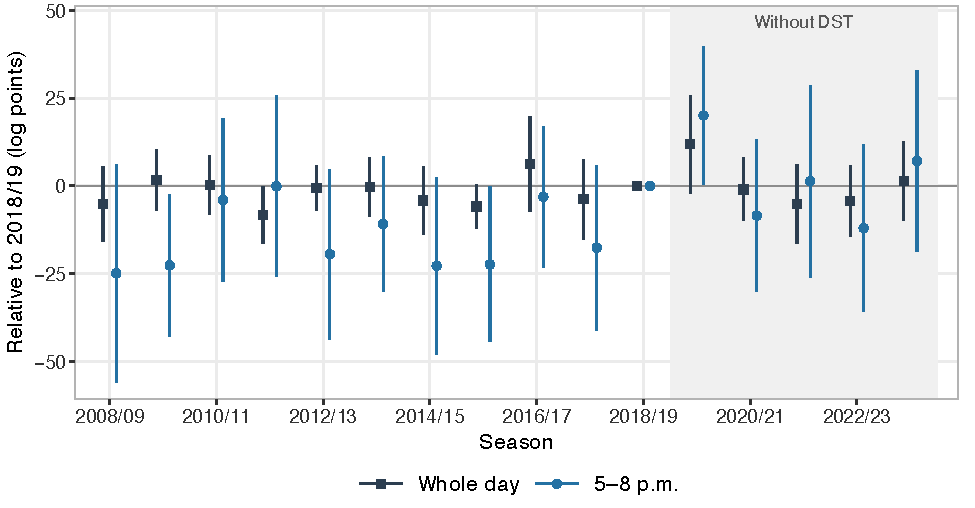
\includegraphics{fig_assault.pdf}
  \caption{Assault deaths, season by season}
  \label{fig:assault}
  \fignote{Deaths from assault in any place, from death certificates.
  Equation~(\ref{eq:main}) by season as in Figure~\ref{fig:event-study}, for
  the whole day and for 5 to 8 p.m. clock time. 95 percent confidence
  intervals.}
\end{figure}

\begin{figure}[p]
  \centering
  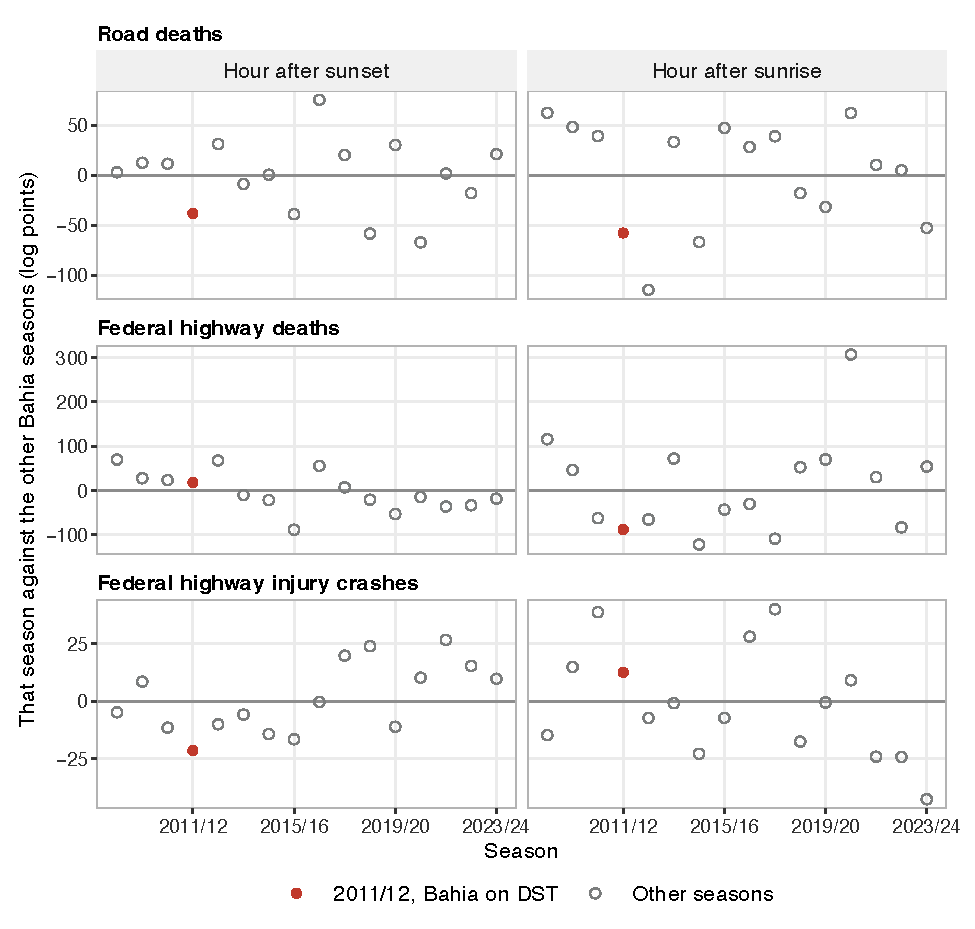
\includegraphics{fig_bahia.pdf}
  \caption{Bahia, the one season it had daylight saving time}
  \label{fig:bahia}
  \fignote{Bahia had DST in 2011/12 only. Each point compares one Bahia season
  with all its other seasons, against the control states, summer window
  against off-season, in the hour after standard-time sunset (left) or
  sunrise (right).}
\end{figure}

\end{document}
